\hypertarget{box_8cpp}{
\subsection{/home/luiggi/Documents/Research/Meshless\_\-RBF/NEW/RBFSoft/examples/01TestKnots/box.cpp File Reference}
\label{box_8cpp}\index{/home/luiggi/Documents/Research/Meshless\_\-RBF/NEW/RBFSoft/examples/01TestKnots/box.cpp@{/home/luiggi/Documents/Research/Meshless\_\-RBF/NEW/RBFSoft/examples/01TestKnots/box.cpp}}
}
Testing the \hyperlink{classBoxKnots}{BoxKnots} class.  




\subsubsection{Detailed Description}
Testing the \hyperlink{classBoxKnots}{BoxKnots} class. 

In this example some features of the class \hyperlink{classBoxKnots}{BoxKnots} are tested. Particularly the function \hyperlink{classKnots_dd136cbe2ce6474885aab4829576472b}{Knots::findNeighbors()} is used to find the neighborhood of a target point. \begin{Desc}
\item[Input ]The {\tt inputBox} file contains the input data required for this program: {\tt hx} length in x-axis; {\tt hy} length in y-axis; {\tt hz} length in z-axis; {\tt Nx} number of points in x-axis; {\tt Ny} number of points in y-axis; {\tt Nz} number of points in z-axis; \end{Desc}
\begin{Desc}
\item[Output]{\tt xyzBox.dat} coordinates of random points; {\tt tarBox.dat} the target point; {\tt neiBox.dat} list of neighbors. \end{Desc}
\begin{Desc}
\item[Post-procesing]You can plot the results using the next command in gnuplot: 

\footnotesize\begin{verbatim}
    % gnuplot> splot "neiBox.dat" w lp, "xyzBox.dat" w p, "tarBox.dat" w p \end{verbatim}
\normalsize
\end{Desc}


 \begin{Image}
\begin{center}
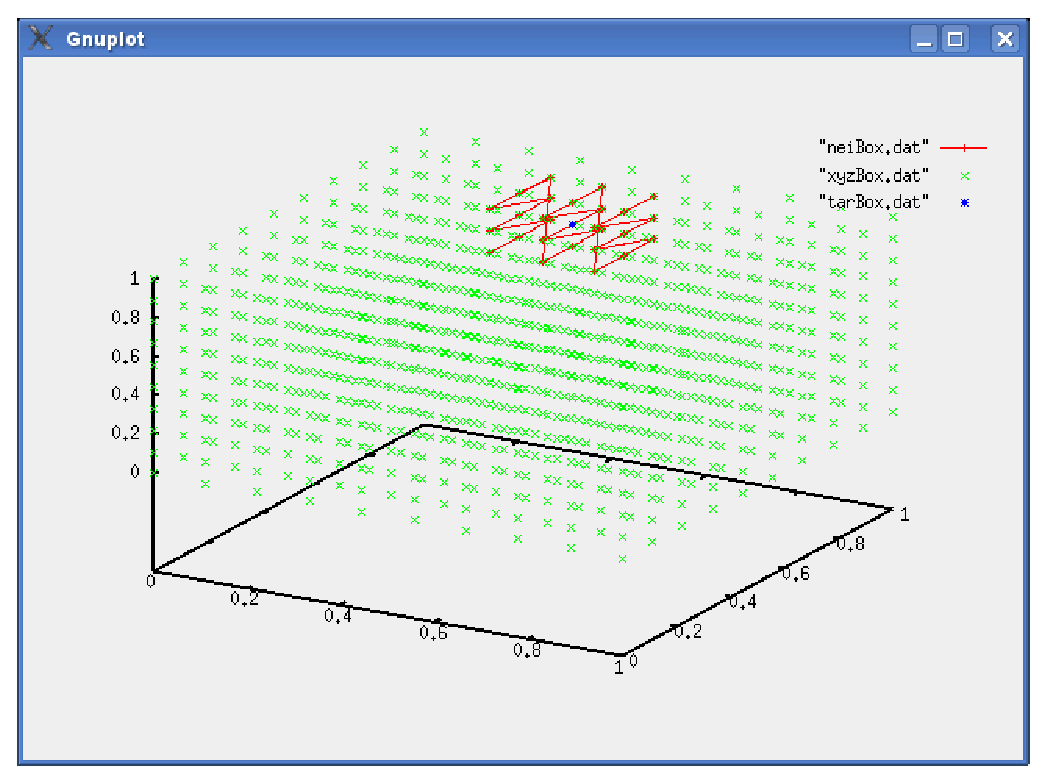
\includegraphics[width=5cm]{boxtest}\caption{Knots, target and neighborhood.}
\end{center}
\end{Image}


\begin{Desc}
\item[Author:]Luis M. de la Cruz \mbox{[} Mon Apr 28 10:31:36 BST 2008 \mbox{]} \end{Desc}


Definition in file \hyperlink{box_8cpp-source}{box.cpp}.